\subsection{Overview: High-level components and their interaction}
The architecture of the system is organized into three major parts: the mobile application, the application server and the database server. These parts respectively represent the logic layers of Presentation, Business and Data access: the mobile app is the user’s workstation and contains the programming that provides the graphical user interface, while the application server acts as server for client requests from the different workstations. Finally, the database server includes the system main database and the DBMS.

\begin{figure}[!h]
	\centering
	\makebox[\textwidth][c]{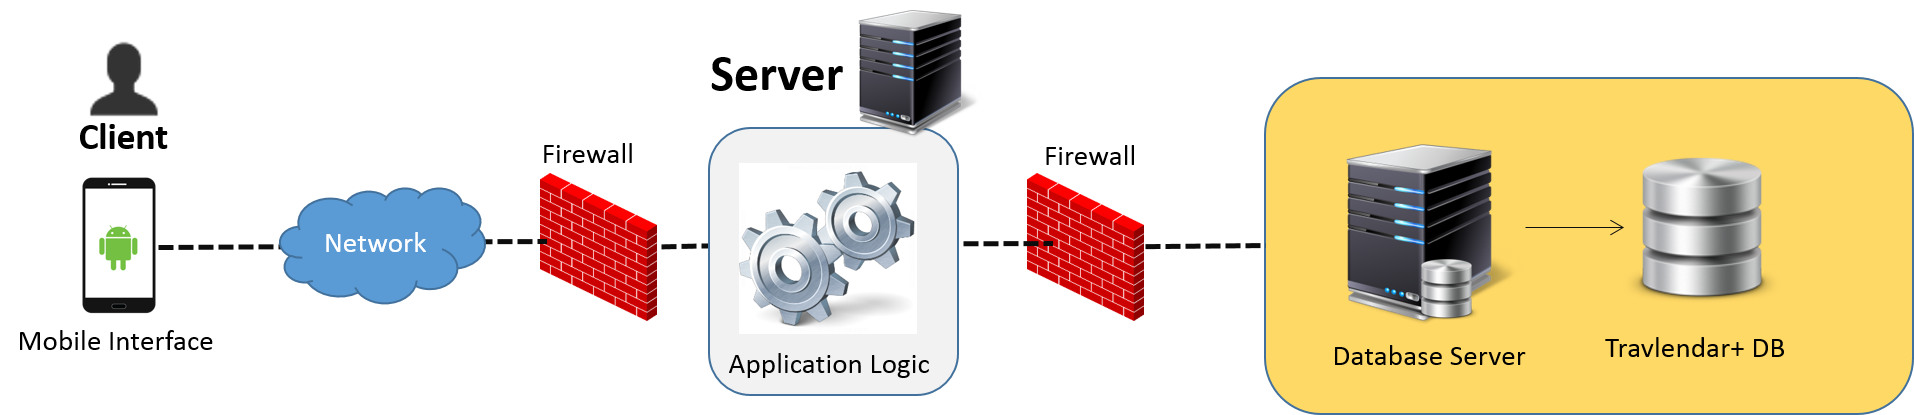
\includegraphics[width=1.2\textwidth]{Images/Architecture/Overview.png}}%
	\caption{System overview}
\end{figure}

\subsection{Component view}
The client side is composed by one main component that implements the functionalities provided to the user in his mobile workstation. The server side architecture is more expanded and it is composed of four main components that represent the application services:\\\\
\textit{Appointment Manager} provides all the functionalities for appointments managing, such as creation and editing of the events or adding of alert. It interacts with the DBMS to store and load appointments data.\\\\
\textit{Travel Manager} is responsible for computing travels and organizing daily schedules. It needs a connection with the DBMS to load info about appointments and makes use of serveral external APIs (such Weather and Maps APIs) to gather data about trace routes, available transport means and weather.\\\\
\textit{Account Manager} manages data about the different Travlendar+ accounts, and allows users to register and log in in the system and saves personal datas. It provides several functionalities to collect info about users settings and preferences.\\\\
\textit{Ticket Manager} contains the essential methods to buy and collect travel tickets. It makes use of APIs of external ticket providers and interacts with the DBMS to load account data and store purchase details.

\begin{figure}[H]
	\centering
	\makebox[\textwidth][c]{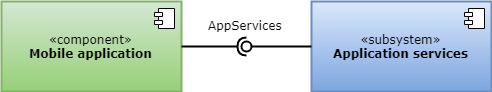
\includegraphics[width=0.8\textwidth]{Images/Architecture/ComponentDiagram1.png}}%
	\caption{Component diagram 1}
\end{figure}
\begin{figure}[H]
	\centering
	\makebox[\textwidth][c]{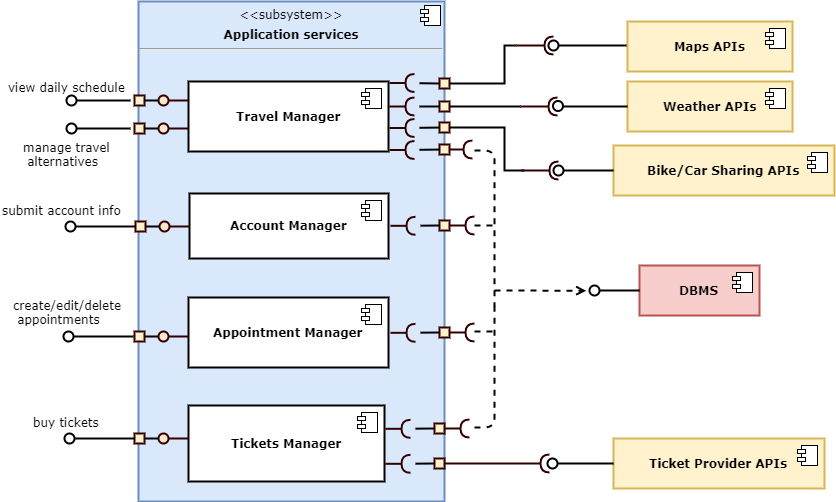
\includegraphics[width=1\textwidth]{Images/Architecture/ComponentDiagram2.png}}%
	\caption{Component diagram 2}
\end{figure}

\subsection{Deployment view}
The architecture of the system is based on JEE framework and consists of three tiers:\\\\
The first tier is the client tier and it is represented by the Travlendar+ user mobile application, running on Android OS. The app is connected via RMI technology to the application server and provides GUI to the user.\\\\
The second tier is the application tier: it is composed by the JBoss AS 7.0.1 Java JEE Server and contains the business logic components of the system. It is connected to the database via jdbc.\\\\
The third tier is the data tier: it is composed by the Database server, that implements MySQL 5.7.19 as relational DBMS.

\begin{figure}[!h]
	\centering
	\makebox[\textwidth][c]{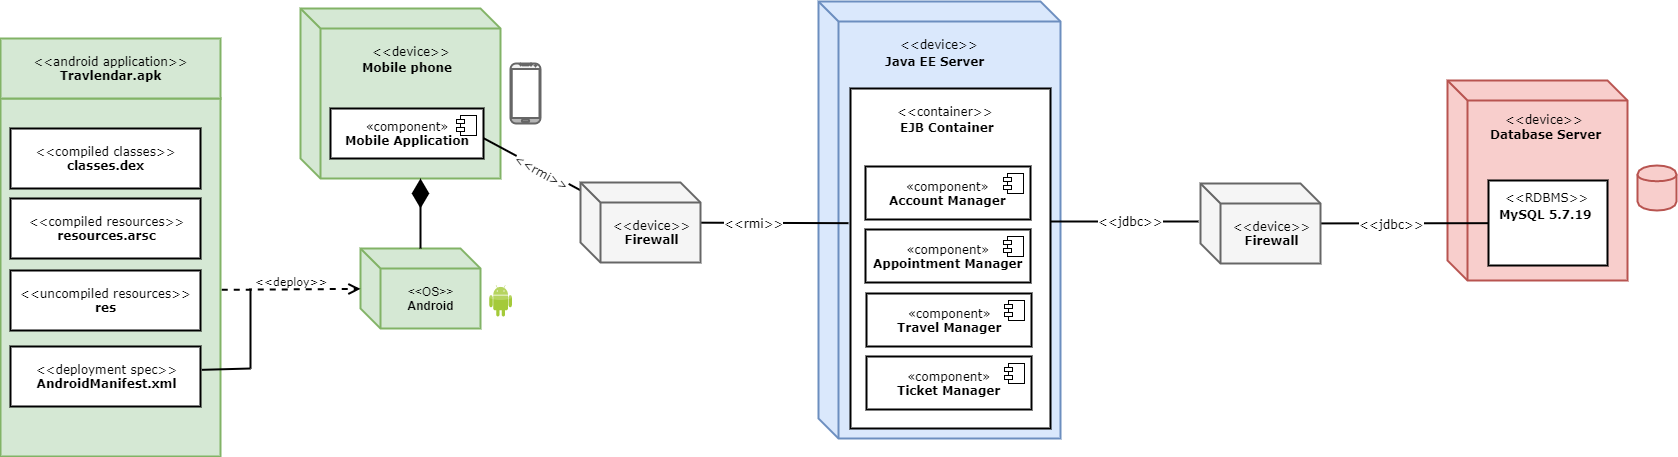
\includegraphics[width=1.2\textwidth]{Images/Architecture/DeploymentDiagram.png}}%
	\caption{Deployment diagram}
\end{figure}
\clearpage

\subsection{Runtime view}
\label{subsec:runtimeView}
\subsubsection{User login}
	\begin{figure}[!h]
		\centering
		\makebox[\textwidth][c]{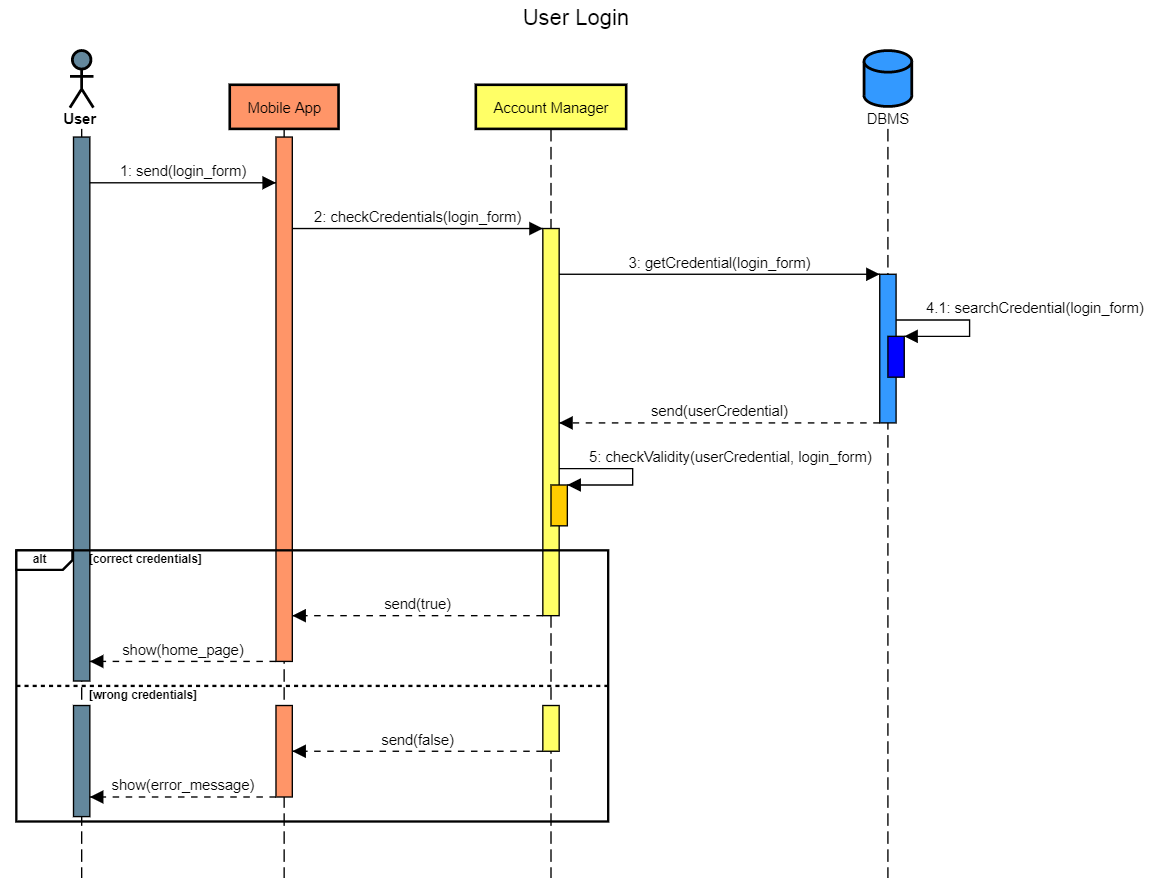
\includegraphics[width=1.2\textwidth]{Images/RuntimeView/UserLogin.png}}%
		\caption{Runtime view: user login}
	\end{figure}
	\clearpage
\subsubsection{Appointment creation}
	\begin{figure}[!h]
		\centering
		\makebox[\textwidth][c]{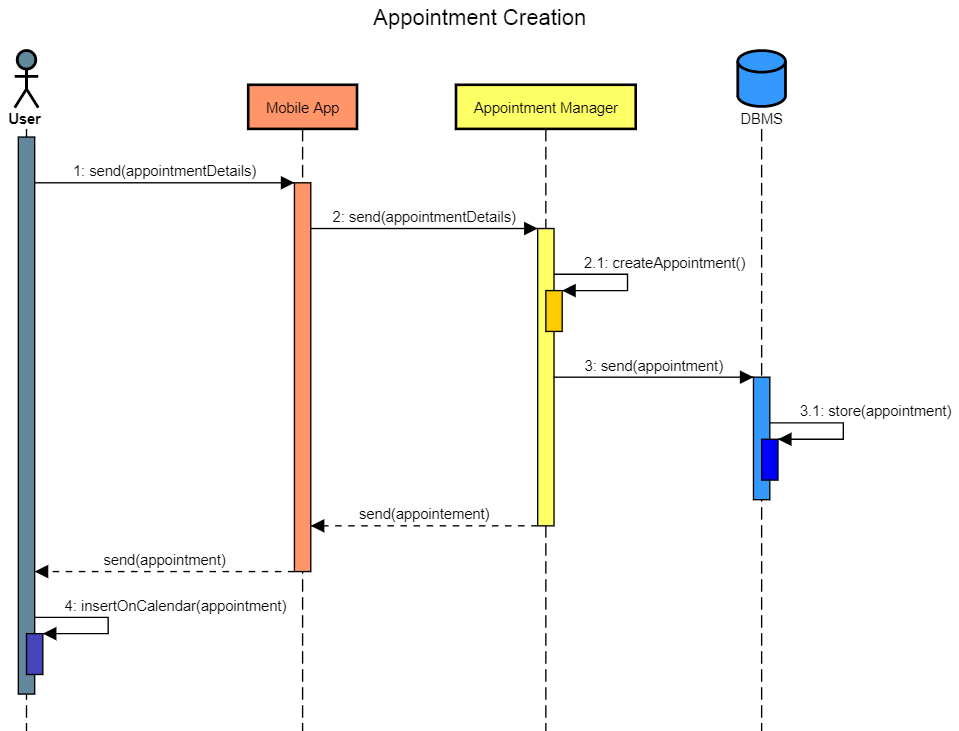
\includegraphics[width=1.2\textwidth]{Images/RuntimeView/AppointmentCreation.png}}%
		\caption{Runtime view: appointment creation}
	\end{figure}
	\clearpage
\subsubsection{Scheduling travel}
	\begin{figure}[!h]
		\centering
		\makebox[\textwidth][c]{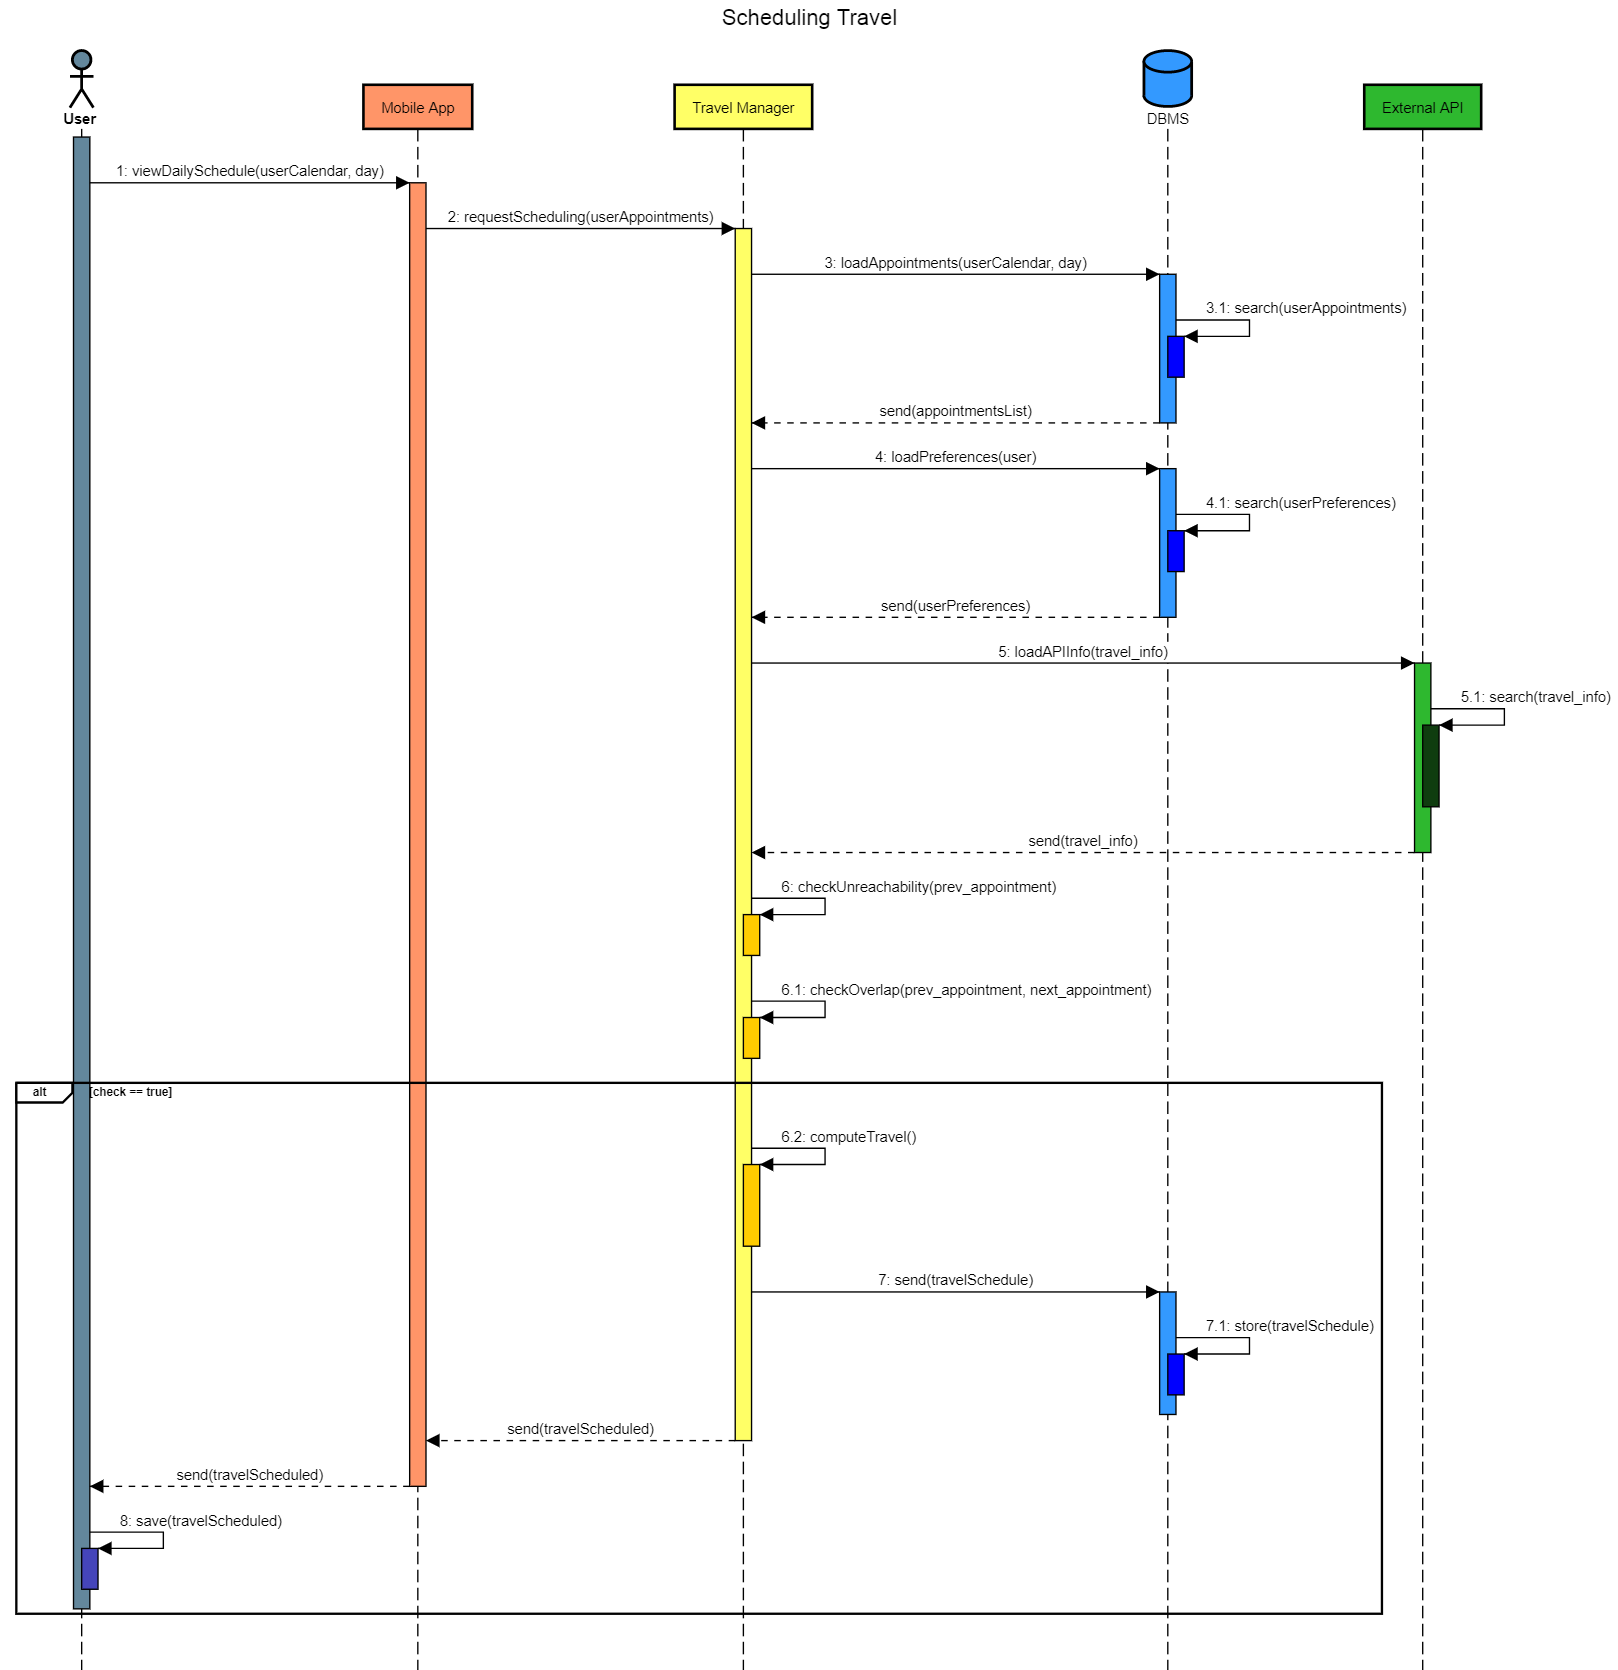
\includegraphics[width=1.2\textwidth]{Images/RuntimeView/SchedulingTravel.png}}%
		\caption{Runtime view: scheduling travel}
	\end{figure}
	\clearpage
\subsubsection{Ticket payment}	
	\begin{figure}[!h]
		\centering
		\makebox[\textwidth][c]{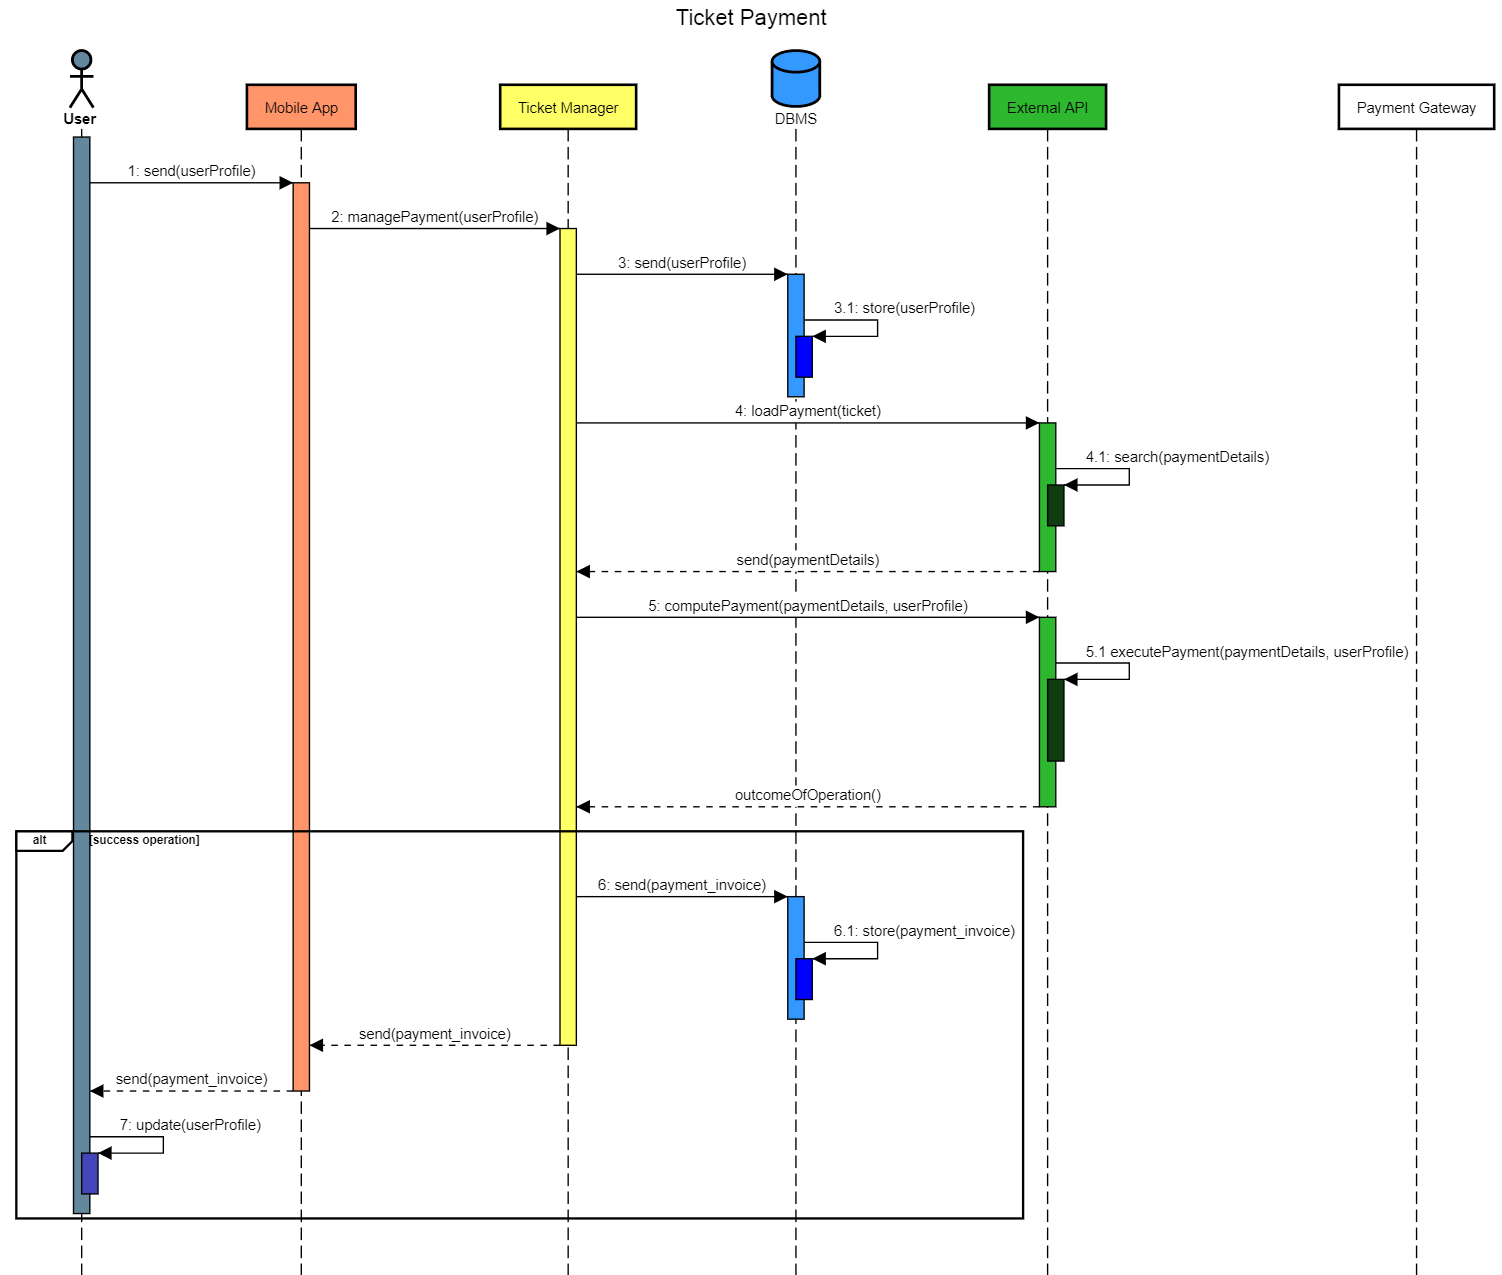
\includegraphics[width=1.2\textwidth]{Images/RuntimeView/TicketPayment.png}}%
		\caption{Runtime view: ticket payment}
	\end{figure}
	\clearpage

\subsection{Component interfaces}
	\begin{figure}[!h]
		\centering
		\makebox[\textwidth][c]{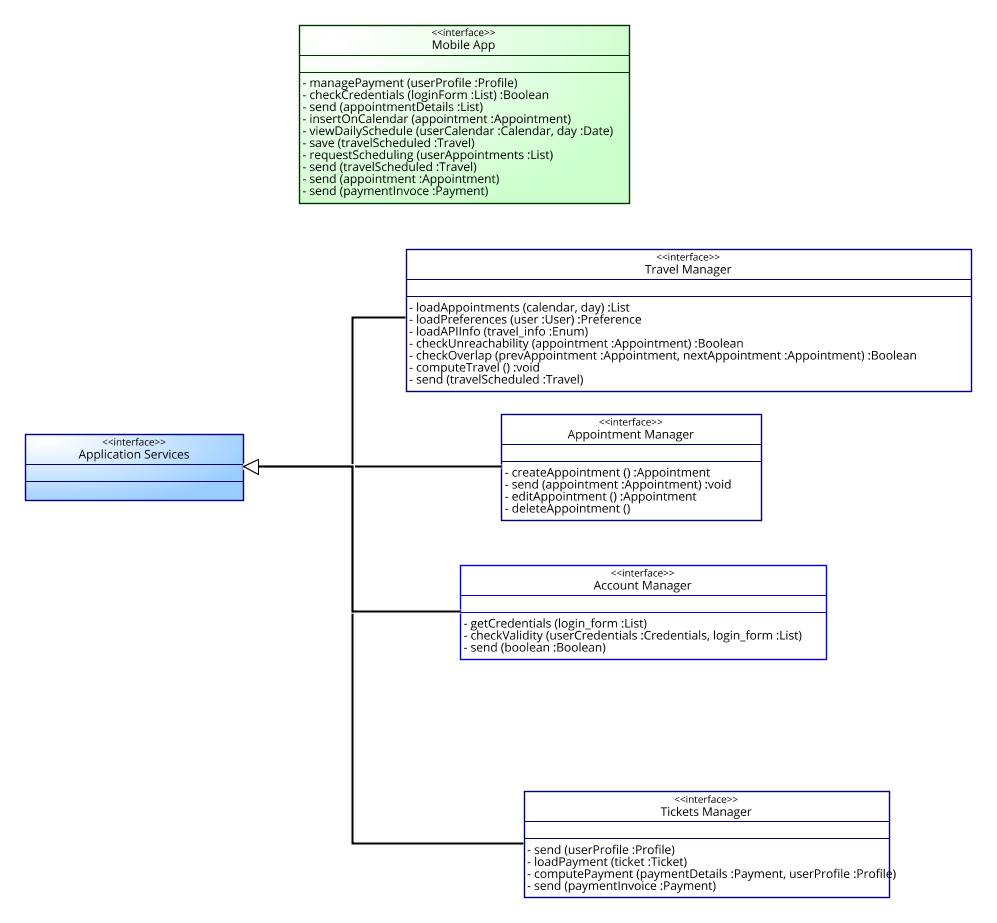
\includegraphics[width=1.2\textwidth]{Images/Architecture/ComponentInterface.png}}%
		\caption{Component interface}
	\end{figure}
	\clearpage

\subsection{Selected architectural styles and patterns}
\begin{itemize}
	\item \textbf{State pattern}: appointments can assume different state, depending on time or concurrency situation.\\ Possible state are: 
		\begin{itemize}
			\item unreachable;
			\item overlapped;
			\item past;
			\item present;
			\item future;
		\end{itemize}
	\item \textbf{Model-view-controller}: usefull to manage interaction between client and application server.
	\item \textbf{Observer pattern}: permits to comunicate in a simple way beetwen server and client, for example to manage notifications
	
\end{itemize}
